% Chapter 6

\chapter{Experimental Results} % Main chapter title

\label{Chapter6} % For referencing the chapter elsewhere, use \ref{Chapter6} 

%----------------------------------------------------------------------------------------
\section{Introduction}
In the previous chapters, we described how DeepMiRNA's architecture is based on two main functional blocks: on one side there is the NN, whose purpose is that of analyzing the selected candidate target sites, while on the other there are the CSSM used during the target prediction step and the a-posteriori filter that tries to refine the predictions. 

To assess these two aspects, we first evaluated the outputs of the NN training process through cross-validation and then investigated its performance using the different candidate site selection methods outlined in chapter \ref{Chapter4}. These comprised the novel (non-canonical) models implemented for this thesis: CSS-6.0:10, CSS-7.0:10 and CSS-7.1:10. Finally, we tested DeepMiRNA’s performance by comparing it against TargetScan\cite{targetscan}, PITA\cite{accessibility_nrg_role} and miRAW \cite{miraw}, which represent the most commonly used target site predictors based on citations.

The experimental results present in this chapter concern the best pipeline configuration for DeepMiRNA. This comprises the use of the MPL network that exhibited an overall better performance than the convolutional model, especially in the identification of negative binding sites. 

There can be many reasons explaining these differences, but we believe that the lack of a consistent dataset of negatively validated binding sites may be the principal cause. 

\section{Neural Network evaluation}
The best performing feed-forward neural network was trained with this parameters:

\begin{itemize}
	\item dropout rate = 0.7
	\item optimizer = Adam as described in chapter \ref{Chapter5}
	\item loss function = binary cross entropy
	\item batch size = 128
	\item number of epochs = 15
\end{itemize}

The above parameters were computed using a validation set of about 10000 examples (20\% of the training set).

Once the best model has been selected, we built a fresh network using the obtained parameters and we trained it holding out the 25\% of the training data for the purpose of testing its performance. This validation presented very good results in terms of predicting both positive and negative sites, with all evaluated metrics resulting in scores well above 0.9 (see figure\ref{fig:network_evaluation}). 

\begin{figure}[hbt!]
	\centering
	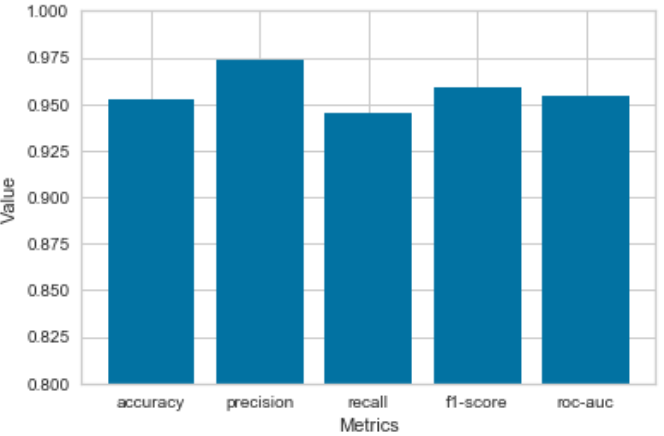
\includegraphics[width=\textwidth]{Figures/network_evaluation}
	\caption{\textbf{Network performance metrics.} To this purpose, we trained the network with the best parameters using 75\% of the training data. The remaining 25\% has been used as a test set. As shown above, all metrics are close to 0.95.}
	\label{fig:network_evaluation}
\end{figure}


\section{The role of the candidate site selection method}
The purpose of using a CSSM is to narrow the search space to simplify the neural network classification task. To investigate the impact of the site selection method, we compared the performances of three different methods as described in chapter\ref{Chapter4}. 

Figure \ref{fig:cssm} summaries the obtained results: all methods reach accuracies between 0.8 and 0.82, these values are computed considering the imbalance of the test set, that is they are calculated as the average of the accuracies on positive and negative samples. CSS-6.0:10 seems to achieve slightly better performances for every metric but precision, compared to the other two methods. The F1-score, which is the harmonic average between precision and recall, shows how well both classes are classified by a particular CSSM. The values obtained are very similar to the accuracy and indicate an ability to effectively predict both negative and positive targets especially for CSS-6.0:10 and CSS-7.0:10.

\begin{figure}[hbt!]
	\centering
	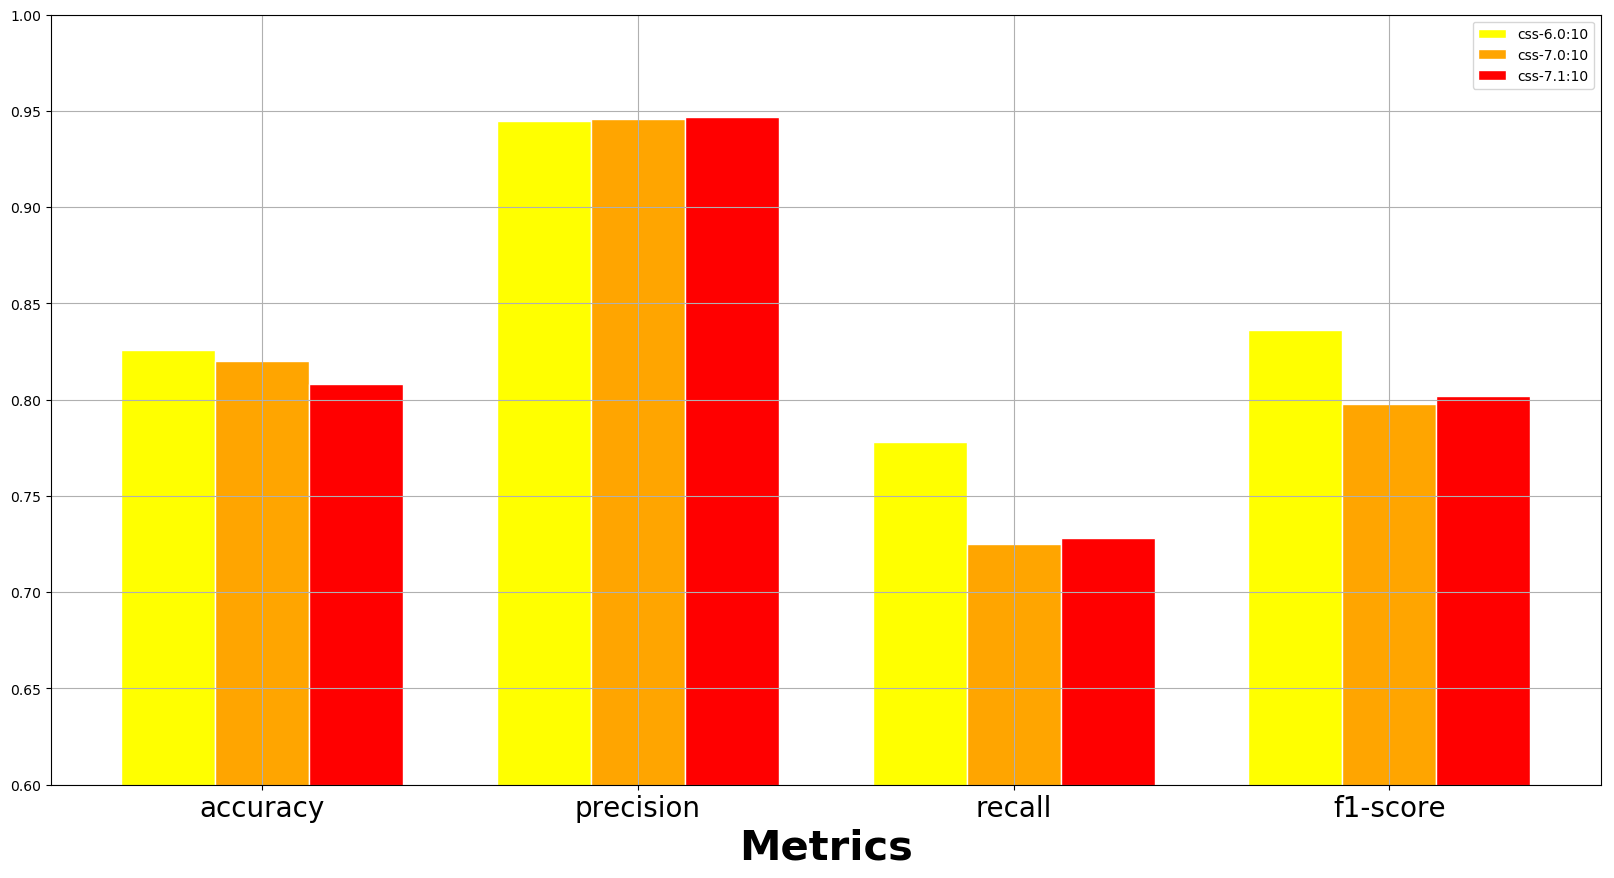
\includegraphics[width=\textwidth]{Figures/cssm_evaluation}
	\caption{\textbf{Evaluation of DeepMiRNA different candidate site selection methods.} Results are evaluated in terms of balanced accuracy, precision, recall and f1-score. The best result was achieved using CSS-6.0:10.}
	\label{fig:cssm}
\end{figure}

Candidates selection also involved the choice of a threshold for the binding energy $th_{duplex}$.  The idea was to only retain duplexes with low free energy and, hence, able to form a stable bond. In order to set this value, we randomly extracted 10 non-overlapping folds from the test set, each composed of $5000$ entries, and we averaged the balanced accuracies obtained by each possible choice. Table \ref{tab:free_energy} shows that the best result has been obtained setting $th_{duplex} = -10$ kcal/mol. 

\begin{table}[h!]
	\caption{\textbf{Free energy threshold evalution.}}
	\label{tab:free_energy}
	\centering
	\begin{tabular}{c c}
		\toprule
		\tabhead{Threshold} & \tabhead{Balanced Accuracy} \\
		\midrule
		0 & 0.79 \\
		-2 & 0.792 \\
		-4 & 0.798 \\
		-6 & 0.824 \\
		-8 & 0.849 \\
		-9 & 0.857 \\
		-10 & \textbf{0.861} \\
		-11 & 0.85 \\
		-12 & 0.835 \\
		-14 & 0.788 \\
		-16 & 0.74 \\
		\bottomrule \\
	\end{tabular}
\end{table}

Higher values produce longer lists of candidate sites and potentially increase the number of false positives, while low values may filter functional binding sites and produce a higher number of false negatives.  



\section{Site accessibility filter}
In order to measure the effect of site accessibility on miRNA target prediction, we tested the best performing pipeline configuration without filtering the network output. While this reduces the computational cost of the whole process, DeepMiRNA becomes slightly more biased towards the prediction of positive sites. However, this is true only for the convolutional model. To underline this difference we report the results obtained with both network models.

Table \ref{tab:sa_filter} shows that using a site accessibility filter (WF) with the MLP network does not improve its prediction performance, in fact, a no filter (NF) configuration achieves slightly better results. This means that the rate of false negatives generated by the filter is higher than the gain derived from the reduction of the false positives. Achieving high precision means that when the network outputs a $1$ it almost never fails, while high values of recall imply the number of false negative is low. These results show that the feed-forward network is very precise in identifying negative binding sites, while it behaves worse with positive targets.  

For the CNN, instead, the filtering steps improves the network ability to predict miRNA's targets correctly. Table \ref{tab:sa_filter} indicates that precision, which is the measure of how confident the system is predicting positive values, and balanced accuracies increase, while recall, that is the fraction of positive instances that have been correctly classified over the total amount of validated positive entries, decreases much slower. 

\begin{table}[h!]
	\caption{\textbf{Results with or without the a-posteriori filter.}}
	\label{tab:sa_filter}
	\centering
	\begin{tabular}{| c | c | c | c | c | c | c | c | c |}
		\hline
		\multirow{2}{4.5em}{\textbf{Classifier}} & \multicolumn{2}{c|}{\textbf{Accuracies}} & \multicolumn{2}{c|}{\textbf{Precision}} & \multicolumn{2}{c|}{\textbf{Recall}} & \multicolumn{2}{c|}{\textbf{F1-score}} \\ 
		\cline{2-9}
		& \emph{NF} & \emph{WF} & \emph{NF} & \emph{WF} & \emph{NF} & \emph{WF} & \emph{NF} & \emph{WF} \\ 
		\hline
		\textbf{Feed-forward} & \textbf{0.827} & 0.82 & 0.936 & \textbf{0.939} & \textbf{0.794} & 0.785 & \textbf{0.840} & 0.838 \\ 
		\hline
		\textbf{CNN} & 0.628 & \textbf{0.652} & 0.649 & \textbf{0.761} & \textbf{0.662} & 0.621 & 0.64 & \textbf{0.681} \\ 
		\hline 
	\end{tabular}
\end{table}

\section{Comparison with other miRNA target prediction tools}

Figure \ref{fig:tools} compares the performance of DeepMiRNA best configuration, which is CSS-6.0:10 without filter, with state of art target prediction software tools TargetScan, PITA and miRAW using the test set defined in chapter \ref{Chapter4}.

For TargetScan we exploited both available configurations: TS conserved which uses an additional feature about interspecies conservation of miRNA and TS non-conserved which does not. For both approaches, the low accuracies seem a consequence of their tendency to misclassify true targets as negative; i.e., despite reporting high precision (> 0.9),
their recall, and hence their F1-score, was low and so was their balanced accuracies.

\begin{figure}[hbt!]
	\centering
	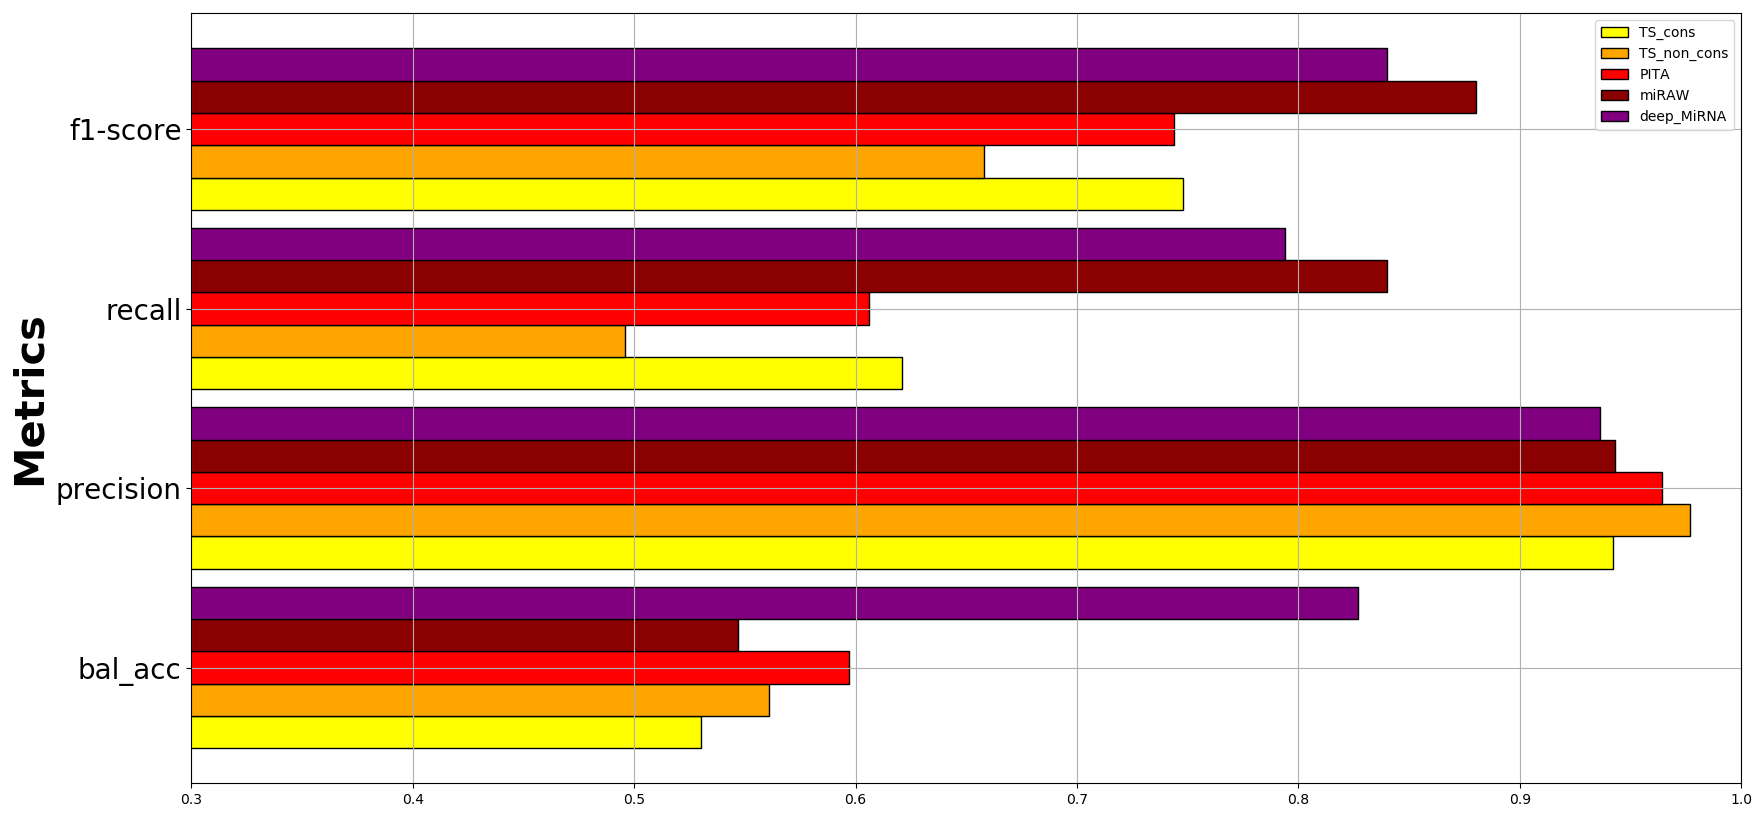
\includegraphics[width=1\textwidth, height=0.5\textheight]{Figures/tools_comparison}
	\caption{\textbf{Comparison of DeepMiRNA with other commonly used prediction tools.} Even though miRAW performs better than DeepMiRNA in most of the metrics, it only has $0.55$ balanced accuracy. This is caused by its poor ability in identifying negative interactions. TargetScan (TS), in both its configurations, and PITA adopt a too conservative approach that inhibits their capacity of recognizing positive duplexes correctly.}
	\label{fig:tools}
\end{figure}

\begin{table}[b!]
	\caption{\textbf{TPR and TNR comparison between miRAW and DeepMiRNA.}}
	\label{tab:metrics}
	\centering
	\begin{tabular}{c c c c c c c c c c}
		\toprule
		\tabhead{Classifier} & \tabhead{NP} & \tabhead{NN} & \tabhead{TP} & \tabhead{FP} & \tabhead{TN} & \tabhead{FN} & \tabhead{TPR} & \tabhead{TNR} & \tabhead{BA} \\
		\midrule
		miRAW & 195825 & 11100 & 84\% & 75\% & 25\% & 16\% & 0.84 & 0.254 & 0.547 \\
		DeepMiRNA & 195825 & 11100 & 80\% & 17\% & 83\% & 20\% & 0.805 & 0.833 & 0.82 \\
		\bottomrule\\
	\end{tabular}
\end{table} 

Conversely, PITA reported better accuracy and F1-score, but still lower than the one achieved by miRAW and DeepMiRNA. According to precision, recall and, hence, F1-score, miRAW performs slightly better than our tool, however the accuracy it achieves is very low (0.55). Balanced accuracy is defined as the average between the true positive (TPR) and the true negative rates (TNR); to explain why miRAW reported such a low value for this metric we can check Table \ref{tab:metrics}.

NP and NN identify respectively the number of positive and negative validated pairs in the test set, while TP, FP, TN and FN indicate the percentage of true/false positive/negative predictions. 
In particular, these values have been computed as the fraction of predicted values of a certain class over the total size of the same class. So, for example, a TP value of $84\%$ states that of all positive samples of the test set $84\%$ were classified correctly, while an FN of $16\%$ indicates that for the negative class 16 samples out of 100 were misclassified. Those values help in giving a feel of what TPR and TNR represent. Finally, BA stands for balance accuracy.
 
MiRAW achieves a true positive rate of $0.84$ indicating its better ability in identifying positives miRNA:mRNA pairs compared to the other tools. However, a large number of negative sites have also been misclassified as positive ($75\%$), meaning that it performed poorly on negative entries. This is confirmed by a very low true negative rate which gives rise to a lower value of balanced accuracy.

Conversely, DeepMiRNA shows a good ability in predicting both classes, even though it tends to be slightly biased towards negative predictions. 

This tendency is reflected in the confusion matrix shown in figure \ref{fig:confusion_matrix} concerning DeepMiRNA's performance over the complete test set.

\begin{figure}[h!]
	\centering
	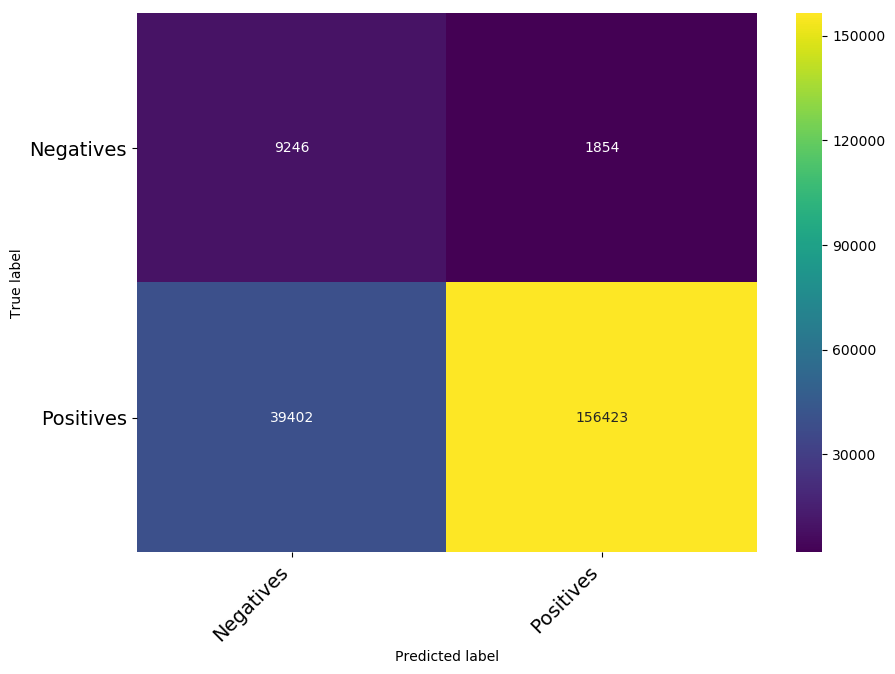
\includegraphics[width=0.7\textwidth, height=0.4\textheight]{Figures/conf_matrix}
	\caption{\textbf{DeepMiRNA Confusion matrix for the test set.} This matrix shows that DeepMiRNA performs well on both classes.}
	\label{fig:confusion_matrix}
\end{figure} 
  


 